\documentclass[tikz,border=8pt]{standalone}
% Shared look for every TikZ diagram. Load with \input{../../tools/tikz-style.tex}
\usepackage[T1]{fontenc}
\usepackage{lmodern}
\renewcommand{\sfdefault}{lmr}  % diagrams use the same serif as the text
\usetikzlibrary{arrows.meta, positioning, shapes.geometric, calc, fit, backgrounds}
\definecolor{cblue}{HTML}{4C78A8}
\definecolor{corange}{HTML}{F58518}
\definecolor{cgreen}{HTML}{54A24B}
\definecolor{cred}{HTML}{E45756}
\definecolor{cpurple}{HTML}{B279A2}
\definecolor{cgrey}{HTML}{6B6B6B}
\tikzset{
  every picture/.style={font=\sffamily, line width=1.2pt},
  box/.style={draw=#1, fill=#1!12, rounded corners=4pt, align=center, inner sep=7pt, minimum height=1.1cm},
  box/.default=cgrey,
  arrow/.style={-{Stealth[length=3mm]}, draw=cgrey, line width=1.4pt},
  title/.style={font=\sffamily\bfseries\Large},
  note/.style={font=\sffamily\small, text=cgrey, align=center},
}
\AtBeginDocument{\hyphenpenalty=10000 \exhyphenpenalty=10000}

\begin{document}
% Section 2.1: one student becomes one training row for the meta-model. The features go into the three base models;
% their predictions become the new row's inputs; the target stays the same.
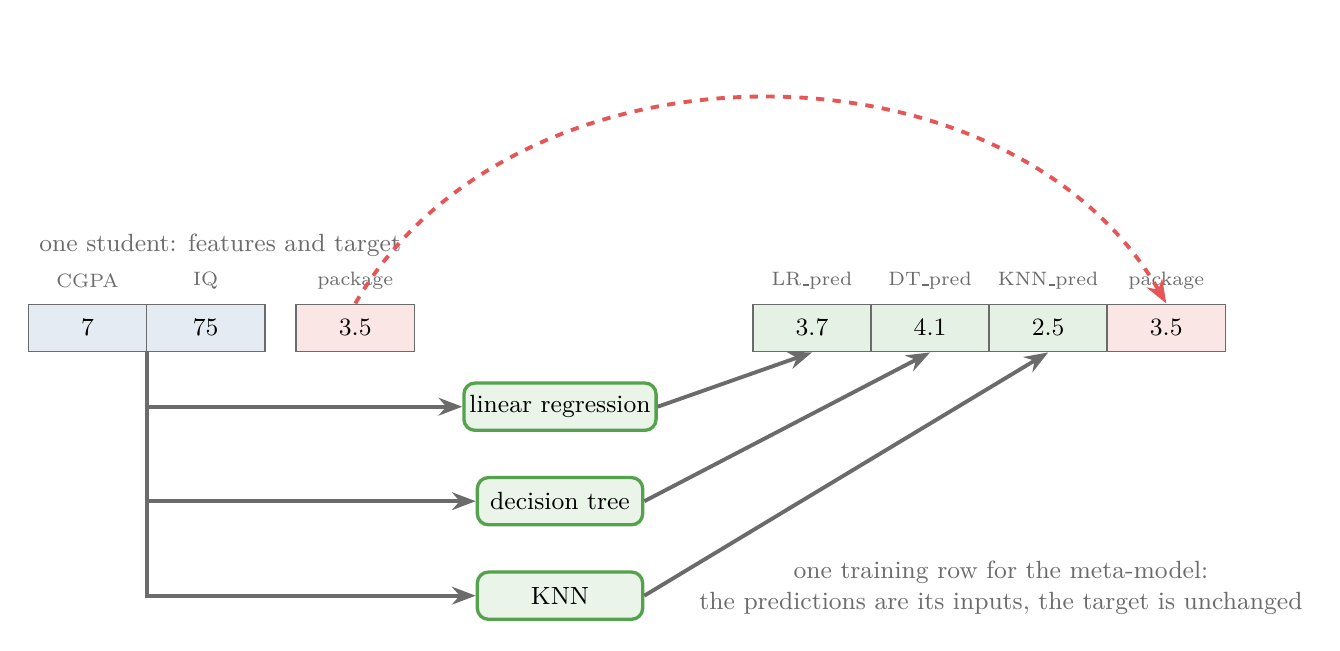
\begin{tikzpicture}[c/.style={draw=cgrey, minimum width=1.5cm, minimum height=0.6cm, font=\sffamily\small, line width=0.6pt},
  h/.style={font=\sffamily\scriptsize, text=cgrey}, m/.style={box=#1, minimum width=2.1cm, minimum height=0.6cm, inner sep=2pt, font=\sffamily\small}]
  \node[h] at (0, 0.6) {CGPA}; \node[h] at (1.5, 0.6) {IQ}; \node[h] at (3.4, 0.6) {package};
  \node[c, fill=cblue!15] (a) at (0, 0) {7}; \node[c, fill=cblue!15] (b) at (1.5, 0) {75}; \node[c, fill=cred!15] (t) at (3.4, 0) {3.5};
  \node[note, anchor=west] at (-0.75, 1.05) {one student: features and target};
  \node[m=cgreen] (m1) at (6.0, -1.0) {linear regression};
  \node[m=cgreen] (m2) at (6.0, -2.2) {decision tree};
  \node[m=cgreen] (m3) at (6.0, -3.4) {KNN};
  \foreach \i in {1,2,3} \draw[arrow] (0.75, -0.3) |- (m\i.west);
  \node[h] at (9.2, 0.6) {LR\_pred}; \node[h] at (10.7, 0.6) {DT\_pred}; \node[h] at (12.2, 0.6) {KNN\_pred}; \node[h] at (13.7, 0.6) {package};
  \node[c, fill=cgreen!15] (p1) at (9.2, 0) {3.7}; \node[c, fill=cgreen!15] (p2) at (10.7, 0) {4.1};
  \node[c, fill=cgreen!15] (p3) at (12.2, 0) {2.5}; \node[c, fill=cred!15] (t2) at (13.7, 0) {3.5};
  \draw[arrow] (m1.east) -- (p1.south); \draw[arrow] (m2.east) -- (p2.south); \draw[arrow] (m3.east) -- (p3.south);
  \draw[arrow, draw=cred, dashed] (t.north) to[out=60, in=120] (t2.north);
  \node[note, align=center] at (11.6, -3.3) {one training row for the meta-model:\\the predictions are its inputs, the target is unchanged};
\end{tikzpicture}
\end{document}
